\section{Introduction}
Computational performance of parallel applications running on parallel processor can be measured in many ways. The elapsed time, price/performance, the speed up, the efficiency are the most commonly used performance measurement metrics. These metrics exhibit significant information on the performance of parallel applications running on parallel processors.

The elapsed time to run a particular job on a given machine is the most significant measurement metric  of performance. The overall time that a program runs on a given machine is known as an elapsed time for that particular program on that specific machine. Price/performance of a parallel system is simply the elapsed time for a program divided by the cost of the machine that ran the job. This metric is particularly useful in buying the machine according to the budget along with the performance requirement. Once the machine is bought; speed-up and efficiency are the measurements that are often used to explore the fact that, how effectively the machine is used with parallel algorithms running on it.

The speed-up is generally measured by running the same program on a varying number of processors. The speed-up is defined as the elapsed time by single processor divided by the time needed on total number of processors. The efficiency metric is related to that of hardware utilization. It is usually defined as

\begin{equation}
e=\frac{T(1)}{pT(p)}
\end{equation}

Efficiency close to unity means that hardware is being used effectively; low efficiency means that you are wasting resources.

We believe, each of these metrics has disadvantages. In fact, there is important information that cannot be obtained
even by looking at all of them. It is obvious that elapsed time should reduce by adding processors, but by how much  the elapsed time would be reduced, speed-up will let us know. Speed-up close to linear is good news, but how close to linear is good enough? Well, efficiency will explore that how the hardware is performing, but we do not have any standard to evaluate the observed efficiency. Our proposed a new metric Serial Fraction, which is intended to answer these questions. Experimental results shows that the new metric Serial Fraction reveals that synchronization overhead, memory contention hinder the performance of the parallel application, which we would not able to observed by the previously known metrics. Our experimental results also shows that our proposed new metric has an important role in determining the performance pattern of parallel application running on parallel processor.

The rest of the paper is organized as follows. Section II describes the related work done on parallel performance metrics. Section III  describes the derivation of the proposed new metric Serial Fraction. Section IV explains the experimental setup, experimental results of the proposed metric for different scenarios and includes explanation of the results. Section V will conclude the paper.

\section{Background}
Several metrics can be used to evaluate the computational behavior of a parallel application. This section describes the most relevant indicators briefly \cite{one, two}.


\textbf{Parallel    Speedup: } Parallel    Speedup   keeps the problem size constant while measuring    the    behavior    of    the    parallel    code    for    a    rising    number    of parallel    jobs. It is     expressed     as     the     ratio     between     the     sequential     execution     time and    the    execution    time    with parallel tasks \cite{WinNT}.

\textbf{Execution    Time: } The    Execution time    is an absolute value represents    the elapsed time for    executing    a    section    of    code.     It     includes user     time, idle     time and    system    time. The execution time     is     the main metric     that     must     be     used     to     compare     the
improvements    due    to    optimizations \cite{WinNT}.

\textbf{Parallel    Efficiency: } The     Parallel     Efficiency     measures     how     efficiently     the     parallel     algorithm     is     executed     in parallel processors. It    is    measured    as    a    ratio    between    the    measured    parallel    speedup    with p processes    and the    maximum    speedup    achievable. A    commonly    accepted    value    is    a parallel    efficient    greater    than    0.5 \cite{WinNT}.

\textbf{I/O    Time    percentage: } The    I/O    Time    percentage    represents    the    time    spent    for    executing    I/O    routines    w.r.t.    the overall    execution    time. The     I/O     Time     percentage     can     be     measured considering     the difference     between     the execution     time     switching     on     and     off     the     I/O     operations, or     computing     the     time     spent with in the I/O    routines.
The    I/O    Time percentage    can    be    included    in    the    serial    fraction    if    the    I/O operations are    executed    by    a    single    parallel    task \cite{WinNT}.

\textbf{Communication Time: } The     communication time     measures     the     time     taken     for     the     communications among parallel    tasks.    It includes    the    time    for    starting    up    the    communication    and data    transferring \cite{WinNT}.

\textbf{Computing Time: } The    computing    time    represents    the    time    spent    for    executing    operations    not    related    to MPI    calls. The     Computing     Time     can     be     measured     indirectly     as     difference     between     the     execution time    of    each    process    and    its    communication    time \cite{WinNT}.

\textbf{Load    Balance: } The    load    balance    measures    how    the    workload    is    distributed    among    the    parallel    tasks. The     Load     Balance     is     measured     as     ratio     between     the     maximum     value     of     the processes computing    time    and    the    average    value \cite{WinNT}.

\textbf{Scaled    Speedup: } The scaled    speedup measures    the    behavior    of    the    parallel    code    for    a    rising    number    of parallel     tasks     by     maintaining     constant     the     grain     size     (i.e.     the     amount     of     computational     load assigned    to    each    parallel    task). The scaled    speedup    is    the    ratio    of    the sequential execution    time    to    the    parallel    execution
time, with ideal    value 1.    A    value    greater    than    1    represents    the    overhead    introduced    by the     communications management     of     the     parallel tasks and the memory    contention \cite{WinNT}.


To the best of our knowledge, no performance metric on Serial Fraction has been published yet though mentioned many times in the prior works on performance measurement. The Serial Fraction    represents the    part    of    the code that is    not executed in    parallel. It is measured as    percentage    of    the    execution time    taken for
the parts of code executed    sequentially    over    the execution    time for    the    whole    application.    In    a    parallel application,     the     sequential     part     of     the application     is identified     by the     code executed     by     only one     process     while     the     others     are     waiting     for completion,     or by     each     process performing the same    computation. In the next section, we will explain how the performance metric equation for Serial Fraction is derived from Amdahl's law.





\section{The Proposed Metric : Serial Fraction}

We will introduce a new metric that has some advantages over the others derived from Amdahl's law \cite{amdahl}. Suppose, 
$T(p)$ is the time needed to run program on $p$ processors. So, speedup, $s$ is defined by


\begin{equation}
s = \dfrac{T(1)}{T(p)}
\end{equation}

The speed-up is then the elapsed time needed by $1$ processor divided by the time needed on $p$ processors.
The efficiency  is defined as follows:

\begin{equation}
e
  = \dfrac{T(1)}{pT(p)}= \dfrac{s}{p}
\end{equation}

To derive our new metric, we start from famous Amdahl's Law which states

\begin{equation}
T(p)= T_s + {\dfrac{T_p}{p}}
\end{equation}
where $T_s$ is time taken by serial part and $T_p$ is the time taken by parallelizable part of the program. So, obviously we get $T(1) = T_s + T_p$.
\\If we define serial fraction:

\begin{equation}
f
  = \dfrac{T_s}{T(1)}
\end{equation}
then the equation (4) becomes
\[T(p)= fT(1)+{\dfrac{T(1)-T_s}{T_p}}
\]
\[T(p)= fT(1)+{\dfrac{T(1)-fT(1)}{T_p}}
\]
So, we get,

\begin{equation}
T(p)=T(1)f+\dfrac{T(1)*(1-f)}{T_p}
\end{equation}
Observe that, if we replace equation (2) in equation (6), then we get,


\begin{equation}
\dfrac{1}{s} = f + \dfrac{1-f}{T_p}
\end{equation}
Solving this equation for $f$, we get our basic metric equation
\[f(1-\dfrac{1}{p})
  = \dfrac{1}{s}-\dfrac{1}{p}
\]
Finally we get our metric equation as follows:

\begin{equation}
f
  = \dfrac{\dfrac{1}{s}-\dfrac{1}{p}}{1-\dfrac{1}{p}}
\end{equation}

Note that s is measured and thus f is an estimated fraction. Amdahl's law does not take into account many practical factors like it assumes that all parallel processors requires the same amount of time. But the serial fraction provided in Amdahl's law might give some meaningful information for even when the parallel processors are not perfectly balanced in time. In the next section, we will present out experimental results on the derived serial fraction and formulate a clear picture which might convey some useful information for performance metric.

\section{Experimental Results}
In this section, we will present our research findings. First we want to mention the experimental environment. We have used Local Area Multicomputer(LAM) message passing environment to process parallel Floyd application which includes 16 single core desktops interconnected by a fast internet of speed 100 Mb/s.

We will explore the findings on the new metric namely, Sfraction (Serial Fraction).  The floyd shortest path finding algorithm \cite{floyd} has been applied in our experimental environment to get result for five case studies in this paper. Floyd shortest path algorithm has been used to derive the shortest path with different number of MPI processes from 1 to 8, with one process per zone. Various performance metrics have been calculated on given data including our new metric, Sfraction to demonstrate the performance on parallel computing. We will compare the Sfraction values found in different case study to find out it's effectiveness. Figure 1 shows the comparison of Sfraction values found in 500, 1000, 2000 and 3000 nodes using one to eight MPI processes.

\begin{figure}
\begin{center}
%\includegraphics[bb=2.0in 2.0in 3in 2in]{sfcompo.eps}
  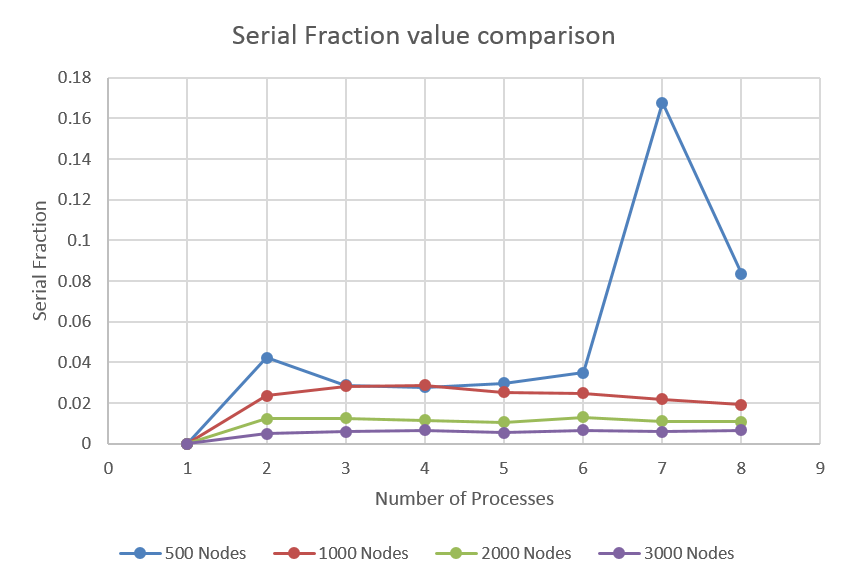
\includegraphics[height=5cm,width=\linewidth]{./image/comp.png}
\end{center}
  \caption{Serial Fraction values for different number of nodes in varying number of processes}
  \label{Fig 1:Serial Fraction Comparison}
\end{figure}


\begin{table}[h!]
\caption{Serial Fraction Feature Comparison[500 nodes, 8 processes]}
\label{tab:Table1}
\centering
% centering table
\begin{tabular}{|c|c|c|c|c|}
\hline
Processes & Time & Speedup & Efficiency & Sfraction\\
\hline
\hline
1&	1.85&	1&	1&	0\\
\hline

2&	0.96&	1.92&	0.959&	0.0423\\
\hline

3&	0.65&	2.84&	0.946&	0.02868\\
\hline

4&	0.5&	3.69&	0.923&	0.02793\\
\hline

5&	0.41&	4.47&	0.894&	0.02972\\
\hline

6&	0.36&	5.11&	0.851&	0.03506\\
\hline

7&	0.53	&3.49	&0.499	&0.16757\\
\hline

8	&0.37	&5.05	&0.631	&0.08361\\
\hline

\end{tabular}
\end{table}

\begin{figure}
\begin{center}
%\includegraphics[bb=2.0in 2.0in 3in 2in]{sfcompo.eps}
  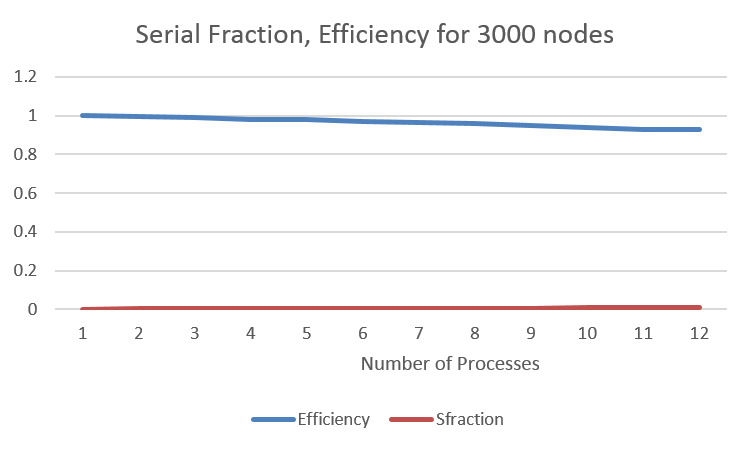
\includegraphics[height=5cm,width=\linewidth]{./image/comp2.png}
\end{center}
  \caption{Serial Fraction Vs Efficiency for 3000 nodes with 12 processes}
  \label{Fig 2:Serial Fraction Comparison}
\end{figure}

From Figure \ref{Fig 1:Serial Fraction Comparison}, we obtain a specific pattern of Sfraction values
as the number of process increases. Serial fraction shows a non decreasing order as the number of processes increases except for the 500 nodes case; though the ratios of non decreasing order behave differently. We can interpret this pattern in a more meaningful way. Usually, number of increasing processes should decrease processing time as well as serial fraction of work but the practical scenario does not always act accordingly. There are certain overheads when parallel processor works together; for example synchronization overhead or memory
contention etc. Hence, increasing the number of processes does not
reduce the serial fraction of work because of the overhead of coordination and synchronization of shared resources related to them. However, from Figure \ref{Fig 1:Serial Fraction Comparison}, we have found a significantly
different behavior for 500 nodes case. To have a deeper look inside 500 nodes case, Table \ref{tab:Table1} representing the experimental result of 500 nodes.

From the determined serial fraction metric values, we can interpret how the speedup and efficiency values changes as the number of process increases in the Floyd application. The reduction of Sfraction values when the processes increases from 2 to 5 probably due to super linear speed up on some processes. The Sfraction value increases  0.02972 to 0.03506 indicates the overhead associated with the process increasing from 5 to 6. However, it is not possible to detect the type of overhead from Sfraction like synchronization overhead or memory contention. From Table \ref{tab:Table1}, we can observe that the Sfraction value of process 7 is showing somehow comparatively large value, might be considered as experimental error. However, We can say that from Figure 1 as all the other experimental value indicating almost the same order in performance measure except node 500.

\begin{table}[h!]
\caption{Serial Fraction Feature Comparison[3000 nodes, 12 processes]}
\label{tab:Table 2}
\centering
% centering table
\begin{tabular}{|c|c|c|c|c|}
\hline
Processes & Time & Speedup & Efficiency & Sfraction\\
\hline
\hline
1&	382.2&	1&	1&	0\\
\hline

2&	191.97&	1.99&	0.995&	0.00453\\
\hline

3&	128.7&	2.97&	0.99&	0.0051\\
\hline

4&	97.51&	3.92&	0.98&	0.00685\\
\hline

5&	78.23&	4.89&	0.977&	0.00584\\
\hline

6&	65.85&	5.8&	0.967&	0.00674\\
\hline

7&	56.59&	6.75&	0.965&	0.00608\\
\hline

8&	49.8&	7.67&	0.959&	0.00606\\
\hline

9&	44.77&	8.54&	0.949&	0.00679\\
\hline

10&	40.67&	9.4&	0.94&	0.00712\\
\hline

11&	37.46&	10.2&	0.927&	0.00782\\
\hline

12&	34.34&	11.13&	0.927&	0.00711\\
\hline

\end{tabular}
\end{table}

In Table \ref{tab:Table 2}, we have given the observed Sfraction values for 3000 nodes running on 12 processes. We can observe the same pattern which we discovered in the Figure \ref{Fig 1:Serial Fraction Comparison} that the Sfraction values are increasing as the number of processes are increasing. It can be interpreted as, synchronization between processes as well as shared resource contention are significant causes behind the increasing number
of serial fraction in the system performance. For further analysis, we have plotted the efficiency and Sfraction values in the Figure \ref{Fig 2:Serial Fraction Comparison}. We can see that the efficiency is decreasing as the number of processes are increasing and on the other hand Sfraction is increasing. This is due to limited parallelism of the running program.

In a nutshell, serial fraction is showing meaningful interpretation of system performance as compared to prior performance metrics though further experiments are necessary to clearly define the reason of change in performance values rather that using certain assumption.

\section{Conclusions and Future Works}
The proposed new metric, Serial Fraction provides the level of parallelization of the code. It sets an upper bound
to the parallel speedup that can be achieved in an ideal parallelization. According to the Amdahl's law, if $s$ is the serial fraction of the code, the maximum speedup achievable with ideal condition is $1/s$. To the best of our knowledge, our metric is the first one to offer a parallel performance measurement using serial fraction which estimates a measure of the parallelization of code in parallel processor systems. This metric provides
an indication of the extent to which a particular code is  parallelized. For a fixed size problem, the efficiency of a parallel computation typically decreases as the number of processors increases. By using the experimentally obtained serial fraction, we can determine if the efficiency decreases due to limited opportunities of parallelism or due to an increase of the algorithmic or architectural overhead. If the value of
the experimentally determined serial fraction is not increasing
with the number of processors, the primary reason for the
poor speedup is the limited opportunity for parallelism. On the
other hand, if the experimentally determined serial fraction is
steadily increasing as the number of processors increases, the
principal reason for the poor speedup is the parallel overhead.

In this paper, we analyzed the experimentally determined serial
fraction to well understand the system behavior by means of
synchronization overhead, load balancing etc. We have used
Floyd parallel application for varying nodes to determine
performance metrics and the effectiveness of the newly derived
metric. Our experimental result shows that serial fraction can
be effectively used in parallel computing system though we
could not determine the reason of experimental error for node
500 case. Further experiments on this metric will be conducted
to have a intense look on the possible cause of errors.







